\documentclass{article}

\usepackage{authblk}
\usepackage{hyperref}
\usepackage{float}
\usepackage{multirow}
\usepackage{graphicx}
\usepackage{subcaption}
\usepackage{amsmath}  % Add the amsmath package
\hypersetup{
    colorlinks=true,
    linkcolor=blue,
    filecolor=magenta,      
    urlcolor=cyan,
}
\providecommand{\keywords}[1]{\small \textbf{Keywords:} #1}

\title{The Role of Macroeconomic Factors and Macro Attention Indices in Forecasting Equity Risk Premia}
\author{Aaron Arauz Baumender (22-748-388) 
\\ Michael Adrian Geiser Pasquel (22-738-645)
\\ Andreas Stavropoulos (22-739-965)
\\ Zhiyi Tang (21-746-763)}
\affil{University of Zurich}
\date{December 2023}

\begin{document}

\maketitle

\begin{abstract} 
\noindent We conduct equity risk premia forecasts (S\&P 500). Our analysis focuses on the utilization of linear and neural network models trained on macroeconomic factors and macroeconomic attention indices.
\end{abstract}

\hfill

\noindent \keywords{Equity risk premia; Macroeconomic factors; Macro economic attention indices; Neural networks; Financial forecast}\\

\newpage

\tableofcontents

\newpage

\section{Introduction}

Equity risk premia, representing the excess return investors expect to receive for holding equities over a risk-free asset, are integral to investment decision-making. The challenge of accurately forecasting these premia has prompted researchers to explore diverse factors, ranging from traditional macroeconomic indicators to emerging metrics like macro attention indices. This study aims to contribute to the predictive modeling landscape by investigating the forecasting capacity of equity risk premia using both linear and neural network models, trained independently with distinct sets of macroeconomic factors and macro attention indices.

\subsection{Background}

Traditional approaches to forecasting equity risk premia have primarily focused on macroeconomic factors such as interest rates, inflation, and economic growth. Concurrently, the burgeoning field of behavioral finance has introduced macro attention indices—quantifiable measures capturing the collective attention of market participants. These indices reflect the market's sensitivity to information flows and the evolving sentiment among investors.

The rationale for this study lies in recognizing the pivotal interplay between macroeconomic factors and macro attention indices in understanding and predicting equity risk premia. By employing two distinct modeling approaches—linear regression models and neural networks—we seek to disentangle the unique contributions of each set of variables, providing a nuanced understanding of their individual and collective impact on forecasting performance.

\subsection{Objectives}

This research has the following key objectives:
\begin{itemize}
  \item Assess the individual predictive capacity of macroeconomic factors in forecasting equity risk premia using linear regression and neural network models.
  \item Evaluate the effectiveness of macro attention indices in predicting equity risk premia through both linear and neural network models.
  \item Investigate the combined predictive power of macroeconomic factors and macro attention indices by developing integrated models.
\end{itemize}

\subsection{Significance of the Study}

The significance of this study extends beyond traditional forecasting methodologies. By employing both linear and neural network models, and considering two distinct sets of variables, we aim to provide a comprehensive analysis that can inform investors, policymakers, and researchers. The findings will contribute insights into the relative strengths and weaknesses of different modeling approaches, ultimately enhancing the understanding of equity market dynamics.

In the subsequent sections, we will delve into a detailed literature review, establish a robust theoretical framework, and conduct empirical analyses to unravel the intricate relationships between macroeconomic factors, macro attention indices, and the forecasting of equity risk premia.

\newpage

\section{Literature Review}

The literature on forecasting equity risk premia spans studies exploring various factors and methodologies. In this section, we review key contributions related to macroeconomic factors, macro attention indices, and their intersection in predicting equity risk premia.

\subsection{Macroeconomic Factors and Equity Risk Premia}

Historically, research emphasized the role of macroeconomic variables in forecasting equity risk premia. Studies by Fama and French (1988) and Goyal and Welch (2003) explored the impact of dividends and book value on equity markets, providing foundational insights into the relationships between traditional macroeconomic indicators and risk pricing.

Recent contributions by Lo and Singh (2003) and Gu et al. (2019) extended this research, employing advanced econometric techniques to analyze non-linear relationships between macroeconomic factors and risk premia. Their findings suggest intricate dynamics between certain macroeconomic variables and risk premia, highlighting the need for sophisticated modeling.

\subsection{Macro Attention Indices and Financial Markets}

The emergence of macro attention indices represents a paradigm shift in understanding how information dissemination influences market dynamics. Studies by Andrei and Hasler (2006) and Nikkien et al. (2006) introduce the concept of macro attention and its role in shaping investor sentiment, capturing collective attention from online and media sources.

Recent research by Ma et al. (2022) shows that incorporating macro attention indices in forecasting models enhances predictive accuracy, especially during heightened market uncertainty. This underscores the importance of considering not only traditional economic indicators but also the broader information environment in forecasting equity risk premia.

\subsection{Integration of Macroeconomic Factors and Macro Attention Indices}

While studies independently explored the impact of macroeconomic factors and macro attention indices, to the best of our knowledge, no papers examine their joint influence on equity risk premia. Individual analyses suggest combining these variables might provide a more robust framework for predicting market movements, emphasizing the need for a holistic approach. This study addresses this gap by employing linear regression models and neural networks to dissect individual and joint contributions to forecasting equity risk premia.

Moreover, we delve into specific macroeconomic indicators, such as inflation rates and interest rates, and assess their interplay with macro attention metrics. This comprehensive analysis aims to uncover nuanced relationships that could enhance our understanding of equity risk premia dynamics.

In the following sections, we establish a theoretical framework, outline the methodology, present empirical findings, and discuss the implications of our research for both academic literature and practical applications.

\newpage

\section{Theoretical Framework}

The theoretical framework guiding this study integrates principles from financial economics, behavioral finance, and the application of machine learning techniques. Our approach to forecasting the S\&P 500 equity risk premia involves a synthesis of traditional economic drivers and contemporary behavioral factors.

\subsection{Market Dynamics Beyond Efficiency}

Contrary to the traditional Efficient Market Hypothesis (EMH), which posits that financial markets rapidly assimilate all available information, our framework acknowledges the existence of market dynamics beyond complete efficiency. We recognize that market anomalies and deviations from efficiency persist, particularly during periods of heightened investor attention. These anomalies challenge the notion of a consistently efficient market and underscore the need for alternative frameworks.

\subsection{Behavioral Finance and Investor Attention}

Incorporating insights from behavioral finance, our framework introduces psychological aspects into financial decision-making. The concept of investor attention emphasizes that market participants may exhibit herd behavior and react to attention-grabbing information, leading to periods of overreaction or underreaction in the market. By integrating macro attention indices in our forecasting models, we account for the role of sentiment and investor attention in shaping market dynamics, acknowledging the limitations of purely rational decision-making assumptions.

\subsection{Neural Networks in Financial Forecasting}

Neural networks provide a flexible framework for capturing complex, non-linear relationships within data. Unlike traditional linear models, which may struggle to capture intricate dynamics, our framework leverages the capabilities of neural networks. Previous studies have demonstrated the effectiveness of neural networks in uncovering patterns that linear models might overlook. By employing neural networks in our analysis, we aim to enhance our ability to model and predict the nuanced interactions between macroeconomic factors and attention-based metrics impacting equity risk premia. This adaptability is particularly valuable in the context of the evolving and dynamic nature of financial markets.

\subsection{Model Specification}

For our study, the equity risk premia (GSPC) will be forecasted using both linear regression and neural network models. The macroeconomic factors (MEF) include:

\begin{table}[H]
\centering
\begin{tabular}{|l|l|p{7.5cm}|}
\hline
\textbf{Variable} & \textbf{Name} & \textbf{Description} \\
\hline
dp & Log Dividend-Price & Represents the proportion of dividends paid by S\&P 500 companies relative to the market price. \\
dy & Log Dividend Yield & Signifies the yield on S\&P 500 dividends, indicating the annual dividend income as a percentage of the market price. \\
dp & Log Earnings-Price & Indicates the proportion of earnings generated by S\&P 500 companies relative to the market price. \\
de & Log Dividend-Payout & Reflects the proportion of earnings paid out as dividends by S\&P 500 companies. \\
rvol & Equity Premium Vol & Measures the variability or volatility in the equity premium over a 12-month period, providing insights into market risk. \\
bm & Book-to-Market Ratio & Represents the ratio of the book value of Dow Jones Industrial Average companies to their market value, indicating the value investors assign to a company's assets. \\
ntis & Net Equity Expansion & Quantifies the net expansion or contraction of equity in the market, considering the 12-month sum of net equity issues by NYSE-listed stocks. \\
tbl & Treasury Bill Rate & Represents the interest rate on three-month Treasury bills in the secondary market, serving as a benchmark for short-term risk-free rates. \\
lty & Long-Term Yield & Signifies the yield on long-term government bonds, reflecting the return on long-term fixed-income securities. \\
ltr & Long-Term Return & Represents the historical return on long-term government bonds, providing insights into past performance. \\
tms & Term Spread & Represents the difference between the long-term yield and the treasury bill rate, offering insights into the slope of the yield curve. \\
dfy & Default Yield Spread & Signifies the spread between Moody's BAA corporate bond yield and Moody's AAA corporate bond yield, indicating the additional yield demanded for lower-rated corporate bonds. \\
dfr & Default Return Spread & Represents the spread between the long-term corporate bond return and the long-term government bond return, reflecting the additional return required for investing in corporate bonds with default risk. \\
infl & Inflation & Calculated from the Consumer Price Index for all urban consumers, using two periods of lagged inflation, reflecting the rate of change in the general price level of goods and services over time. \\
\hline
\end{tabular}
\caption{Macroeconomic Factors (MEF) for Equity Risk Premia Forecasting.}
\label{tab:MEF}
\end{table}

The macro attention indices (MAI) include:

\begin{table}[H]
\centering
\begin{tabular}{|l|l|p{7.5cm}|}
\hline
\textbf{Variable} & \textbf{Name} & \textbf{Description} \\
\hline
credit\_rating & Credit Rating & Reflects entities' creditworthiness, influencing investor risk perceptions; a higher credit rating indicates lower default risk. \\
gdp & Gross Domestic Product & Represents total goods and services value within a country, a key indicator of economic health. \\
house\_mkt & House Market & Captures housing market trends, providing insights into broader economic conditions. \\
inflation & Inflation & Measures the percentage change in the general price level, influencing purchasing power and monetary policy. \\
monetary & Monetary & Encompasses attention on monetary policy, including interest rates and central bank decisions. \\
oil & Oil & Reflects attention on the oil market, crucial for understanding energy-related economic trends. \\
unemp & Unemployment Rate & Captures attention related to employment trends and economic stability. \\
usd & US Dollar & Reflects attention on the U.S. dollar, impacting international trade and economic conditions. \\
\hline
\end{tabular}
\caption{Macro Attention Indices (MAI) for Equity Risk Premia Forecasting.}
\label{tab:MAI}
\end{table}

The S\&P 500 (GSPC) equity risk premia include:
\begin{table}[H]
\centering
\begin{tabular}{|l|l|p{7.5cm}|}
\hline
\textbf{Variable} & \textbf{Name} & \textbf{Description} \\
\hline
GSPCprem & Equity Risk Premia  & Reflects the excess return an investor expects to receive from holding equities (stocks) compared to a risk-free (government bonds). \\
\hline
\end{tabular}
\caption{S\&P 500 (GSPC) Equity Risk Premia.}
\label{tab:GSPC}
\end{table}

These variables form the basis for our models, allowing us to independently assess the predictive capabilities of linear regression and neural network models. In the subsequent section, we detail the methodology employed for model implementation and evaluation.

\newpage

\section{Methodology}

Forecasting GSPC equity risk premia involves the application of both linear regression and neural network models using the identified MEF and MAI data. The aim is to independently assess the predictive capabilities of these models and understand how the inclusion of behavioral and attention-based metrics enhances forecasting accuracy.

\subsection{Data Management}

The historical data is collected over a time period of 34 years (1985 to 2018) and with three different frequencies (daily, monthly, quarterly). The datasets are organized to align with the time series nature of financial and economic variables, ensuring chronological order for proper model training and evaluation.

\subsubsection{Data Collection (raw data)}
  
MEF monthly and quarterly raw data is collected from powder197/Goyal-and-Welch-2008- Github repository. This raw data contains the following information: "date", "index", "lag\_index\_1", "d12", "e12", "bm", "tbl", "aaa", "baa", "lty", "ntis", "infl", "ltr", "corpr", and "svar". This information is used in a later stage to construct the 14 macroeconomic factors.

MEF daily raw data is implied from MEF monthly raw data. More specifically, daily "infl", "ltr", and "corpr" variables are implied from monthly data as follows: $\text{ddp} = (1+\text{mdp})^{1/\text{ndm}}-1$, were $\text{ddp}$ stands for daily data point, $\text{mdp}$ stands for monthly data point, and $\text{ndm}$ means number of days in month. 
Daily "d12", "e12", "bm", "tbl", "aaa", "baa", "lty", and "ntis" variables are computed as linear interpolations between monthly data points. Lastly, daily "svar" varialbe is simply calculated as $(\text{mdp}/\text{ndm})$, i.e. prorated data through the month.

MAI daily and monthly raw data is collected from charlesmartineau/mai\_rfs Github repository. This raw data contains the following information: "date", "credit\_rating\_ni", "gdp\_ni", "house\_mkt\_ni", "inflation\_ni", "monetary\_ni", "oil\_ni", "unemp\_ni", "usd\_ni", "credit\_rating\_wi", "gdp\_wi", "house\_mkt\_wi", "inflation\_wi", "monetary\_wi", "oil\_wi", "unemp\_wi", and "usd\_wi". Columns ending with "\_ni" and "\_wi" correspond to information provided by the New York Times and Wall Street Journal, respectively. This information is used in a later stage to construct the eight macro attention indexes.

MAI quarterly raw data is implied from MAI monthly raw data.

GSPC daily, monthly, and quarterly raw data is collected from Yahoo Finance. This raw data contains the following information: "date", "GSCP"	"lead\_GSCP\_1M", "rfr", "lead\_date". This information is used in a later stage to construct the equity risk premia.

\subsubsection{Data Cleaning (interim data)}

The collected data undergoes preprocessing steps to improve the quality and compatibility of the input features. This process specifically addresses missing values in the MAI raw databases.

To illustrate the calculation of MAI daily, monthly, and quarterly interim data, let's consider the "credit\_rating" variable as an example. If "credit\_rating\_ni" is $0$ while "credit\_rating\_wi is not $0$, the $0$ value of "credit\_rating\_ni" is replaced with the value of "credit\_rating\_wi". Conversely, if "credit\_rating\_wi" is $0$ but "credit\_rating\_ni" is not $0$, the $0$ value of "credit\_rating\_wi" is replaced with the value of "credit\_rating\_ni". In the case where both "credit\_rating\_ni" and "credit\_rating\_wi" are $0$, we retain the previous values of both variables, respectively. This approach is rooted in the rationale that if one journal (but not both) fails to produce the "credit\_rating" index, it indicates that no relevant news related to credit rating was published in that specific journal. In such instances, the other magazine contains updated information embedded in the index. However, when both journals fail to produce the "credit\_rating" index, it suggests that no change in credit rating information was released. Consequently, we can safely assume that the previous information remains unchanged, reflecting a status quo in the index.

MEF and GSCP data require no interim treatment.

\subsubsection{Data Processing (processed data)}
The preprocessed data is used to construct the data for model training.

MEF processed data consists of "date" and the 14 macroeconomic factors. The calculations are as follows:
\begin{equation*}
    \text{dp} = \log{(\text{d12})} - \log{(\text{index})},
\end{equation*}
\begin{equation*}
    \text{dy} = \log{(\text{d12})} - \log{(\text{lag\_index\_1})},
\end{equation*}
\begin{equation*}
    \text{ep} = \log{(\text{e12})} - \log{(\text{index})},
\end{equation*}
\begin{equation*}
    \text{de} = \log{(\text{d12})} - \log{(\text{e12})},
\end{equation*}
\begin{equation*}
    \text{tms} = \text{lty} - \text{tbl},
\end{equation*}
\begin{equation*}
    \text{dfy} = \text{baa} - \text{aaa},
\end{equation*}
\begin{equation*}
    \text{dfr} = \text{corp} - \text{ltr}.
\end{equation*}
All other factors, namely rvol, bm, ntis, tbl, lty, and ltr, are directly found from the corresponding columns in the interim data.

MAI processed data consists of "date" and the eight macro attention indexes. The calculation of the index consists of a simple average between the corresponding columns ending with "\_ni" and "\_wi". As an example, "credit\_rating" is computed as follows:
\begin{equation*}
    \text{credit\_rating} = \frac{\text{credit\_rating\_ni}+\text{credit\_rating\_wi}}{2}.
\end{equation*}

GSCP processed data consists of "date" and "GSCPprem" columns. The latter is constructed from interim data as follows:
\begin{equation*}
    \text{GSCPprem} = 100 \times \frac{\text{lead\_GSCP\_1M - \text{GSCP}}}{\text{GSCP}} \times \frac{360}{\text{lead\_date}-\text{date}} - \text{rfr}.
\end{equation*}

\subsection{Model Training}

Two distinct approaches are employed for model training: linear regression and neural network models. For linear regression, the relationship between the GSCP equity risk premia and the MEF/MAI data is modeled using the standard linear regression equation. The coefficients are estimated using gradient decent with Ridge regularization to capture the linear relationships between the variables.

For neural network models, a feedforward neural network architecture is employed. The network is designed with input layers corresponding to the MEF/MAI data sets, hidden layers for capturing non-linear relationships, and an output layer for predicting the GSCP equity risk premia. The network is trained using Adam optimizer, learning rate $0.0001$, epochs $10$, and batch size $32$, two hidden layers (the first one with $64$ neurons, the second one with $32$ neurons), and dropout layers.

The performance of the models is evaluated using Root Mean Squared Error (RMSE).

\subsection{Comparison and Interpretation}

The results from the linear regression and neural network models, expressed in terms of RMSE, are compared to understand their relative strengths and weaknesses in forecasting equity risk premia. Both sets of economic data-MAI and MEF data-are used independently and also combined in order to evaluate the predictive capacity of different combinations. The target variable is the $1$-month GSPC equity risk premia, using as daily and monthly frequency.

\newpage

\section{Empirical Analysis}

The empirical analysis involves implementing the models specified in the methodology section to forecast the $1$-month GSPC equity risk premia based on the selected macroeconomic factors (MEF) and macro attention indices (MAI). For this, we use daily and monthly data from both sets of economic data.

The findings from the analysis provide insights into the effectiveness of linear regression and neural network models in predicting equity risk premia and the impact of attention-based metrics.

\subsection{Data Overview}

In this study, we use six datasets. The table below (Table \ref{tab:Datasets}) shows the characteristics of the datasets.

\begin{table}[H]
\centering
\small
\begin{tabular}{|c|c|c|c|c|}
\hline
Dataset & \begin{tabular}[c]{@{}c@{}}Number of\\ vairiables\end{tabular} & Frequency & Time Period & \begin{tabular}[c]{@{}c@{}}Number of\\ samples\end{tabular} \\ \hline
MEF Daily & 14 & Daily & 1985/01/02-2018/12/31 & 8523 \\ \hline
MAI Daily & 8 & Daily & 1985/01/02-2018/12/31 & 8523 \\ \hline
MKT Daily & 1 & Daily & 1985/01/02-2018/12/31 & 8523 \\ \hline
MEF Monthly & 14 & Monthly & 1985/01/31-2018/12/31 & 408 \\ \hline
MAI Monthly & 8 & Monthly & 1985/01/31-2018/12/31 & 408 \\ \hline
MKT Monthly & 1 & Monthly & 1985/01/31-2018/12/31 & 408 \\ \hline
\end{tabular}
\caption{Description of Datasets used for model training.}
\label{tab:Datasets}
\end{table}

\subsection{Model Implementation}

\subsubsection{Linear Regression Model}

The linear regression model is implemented using the identified macroeconomic factors and macro attention indexes as independent variables. The model is trained on a subset of the dataset, and the coefficients are estimated to establish the linear relationship with the dependent variable.

\subsubsection{Neural Network Model}

The neural network model is implemented using a feedforward neural network architecture. The design of the network includes input layers for MEF and MAI, hidden layers for capturing non-linear relationships, and an output layer for predicting equity risk premia. The model is trained on the dataset, adjusting weights and biases through an optimization process.

\subsection{Results}

\subsubsection{Performance evaluation}

The average root mean square error (RMSE) of eight different models (two types of model on four datasets) is tested on ten different random train-test splits of each dataset.

\begin{table}[H]
\centering
\begin{tabular}{|c|c|c|}
\hline
\textbf{Model} & \textbf{Input Data} & \textbf{RMSE on Test Set} \\ \hline
\multirow{4}{*}{Linear Model} & MEF Daily & 53.243 \\ \cline{2-3} 
 & MAI Daily & 54.677 \\ \cline{2-3} 
 & MEF Monthly & 54.307 \\ \cline{2-3} 
 & MAI Monthly & 53.571 \\ \hline
\multirow{4}{*}{NN Model} & MEF Daily & 51.660 \\ \cline{2-3} 
 & MAI Daily & 51.650 \\ \cline{2-3} 
 & MEF Monthly & 42.794 \\ \cline{2-3} 
 & MAI Monthly & 42.596 \\ \hline
\end{tabular}
\caption{Comparison of RMSE of different models.}
\label{tab:RMSE}
\end{table}

\subsubsection{Predictions}

The figures below elucidates the evident disparities between the actual values and the forecasts generated by our trained models. Specifically, we illustrate this phenomenon by examining the linear model and the neural network model applied to the MAI monthly data. 

\begin{figure}[H]
  \centering
  \begin{subfigure}{0.48\linewidth}
    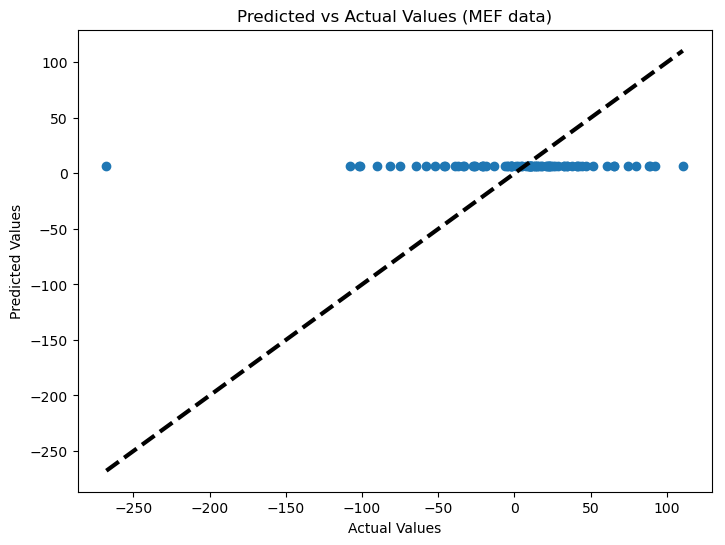
\includegraphics[width=\linewidth]{predvstrue_LM_MAI_M.png}
    \caption{Linear model}
  \end{subfigure}
  \hfill
  \begin{subfigure}{0.48\linewidth}
    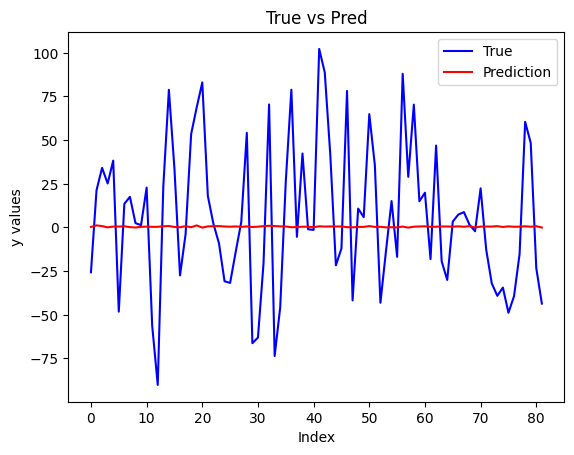
\includegraphics[width=\linewidth]{predvstrue_NN_MAI_M.png}
    \caption{Neural network model}
  \end{subfigure}
  \caption{Predicted vs Actual Values, predicted from MAI monthly data.}
  \label{fig:predvstrue}
\end{figure}

\noindent The generalization capability of the models is also not good enough. The RMSEs on the training sets are much better than those on the test sets.

\begin{figure}[H]
    \centering 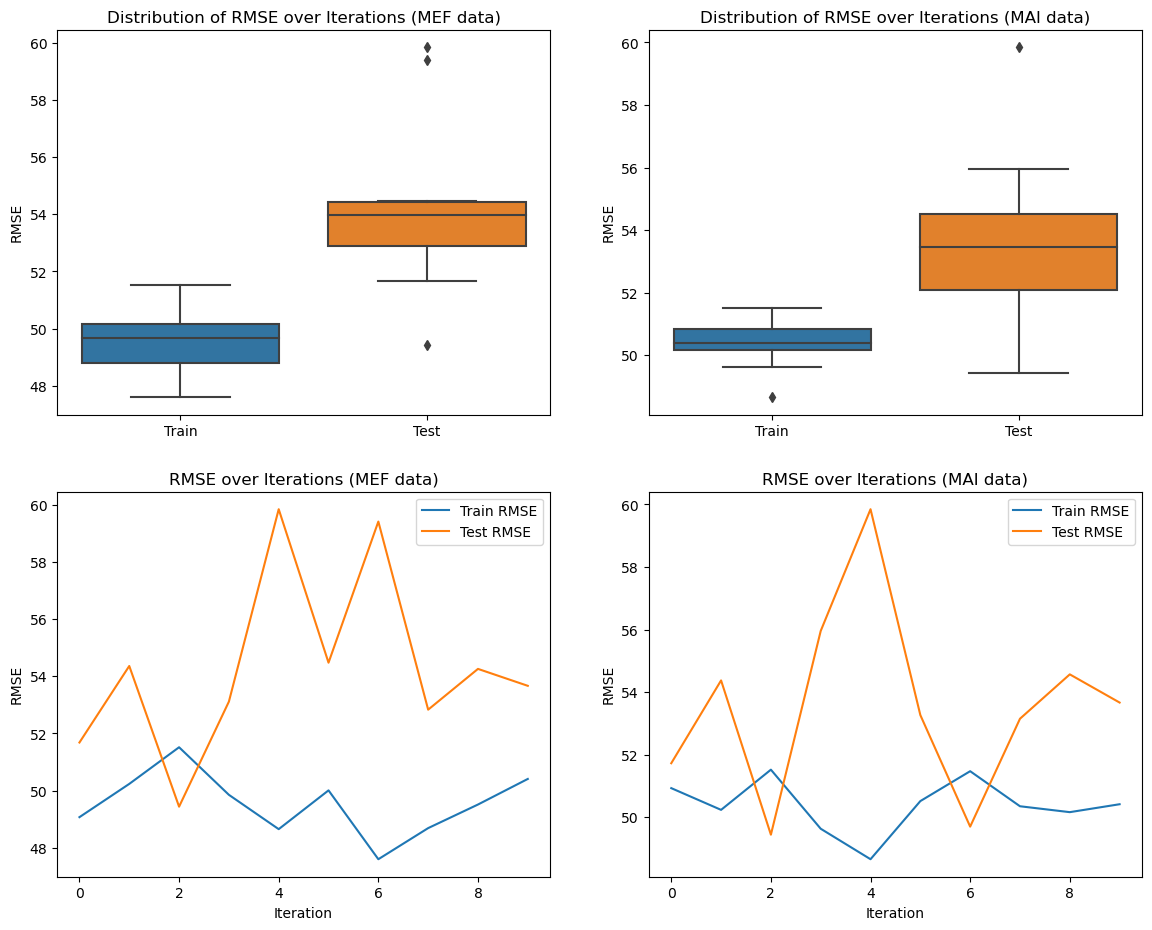
\includegraphics[width=1\linewidth]{Distribution of RMSE_Linear_M.png}
    \caption{Distribution of RMSE over iterations, linear models on monthly data.}
\end{figure}

\begin{figure}[H]
  \centering
  \begin{subfigure}{0.48\linewidth}
    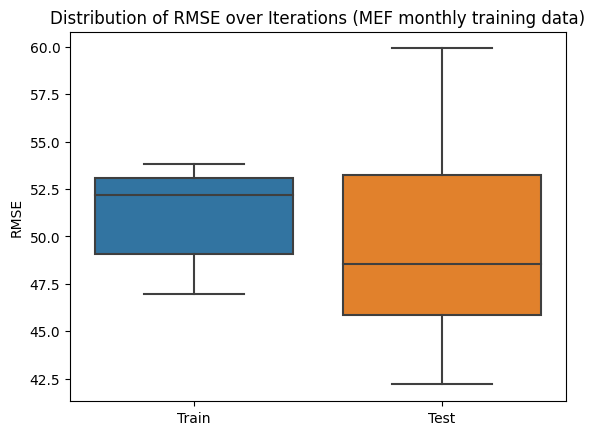
\includegraphics[width=\linewidth]{Distribution of RMSE_NN_MEF_M.png}
    \caption{MEF monthly.}
  \end{subfigure}
  \hfill
  \begin{subfigure}{0.48\linewidth}
    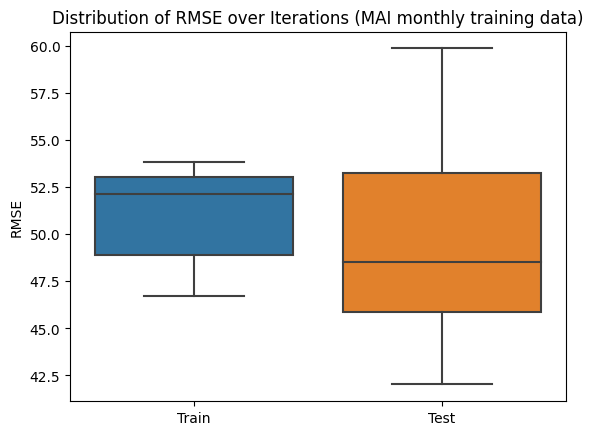
\includegraphics[width=\linewidth]{Distribution of RMSE_NN_MAI_M.png}
    \caption{MAI monthly.}
  \end{subfigure}
  \caption{Distribution of RMSE over iterations, NN models on monthly data.}
\end{figure}

\noindent Despite the substantial variations between predictions and actual values, it is noteworthy that the models still exhibit a discernible capacity to anticipate fluctuation trends.

\subsection{Comparison and Interpretation}

\subsubsection{Model Selection}
The table presented in chapter 5.3.1 (Table \ref{tab:RMSE}) clearly illustrates the superior performance of neural network models compared to linear regression models across all datasets. The RMSE of neural network models is approximately 17 units lower than that of linear models. Neural networks excel in predictive accuracy, making them more robust for real-world applications.

\subsubsection{Data Selection}
Meanwhile, the linear models offer insights into the impact of individual factors on equity risk premia through coefficient examination and significance testing, which are hard to get from the "black box" of NN models. Utilizing the \href{https://baumender11.shinyapps.io/Alpha/}{interactive Shiny app} facilitates a lucid visualization of the impact of various features and temporal ranges on predictive outcomes. Users are afforded the flexibility to select any permutation of the 14 MEF variables, the 8 MAI variables, temporal spans ranging from January 1, 1985, to December 31, 2018, and temporal frequencies at daily, monthly, or quarterly intervals. The MEF model results are denoted by blue lines, the MAI model results by green lines, and the veritable values by the red line.

Here we employ two cases on quarterly data as illustrative examples. With lower frequency, the lines are easier to identify.

\begin{figure}[H]
    \centering 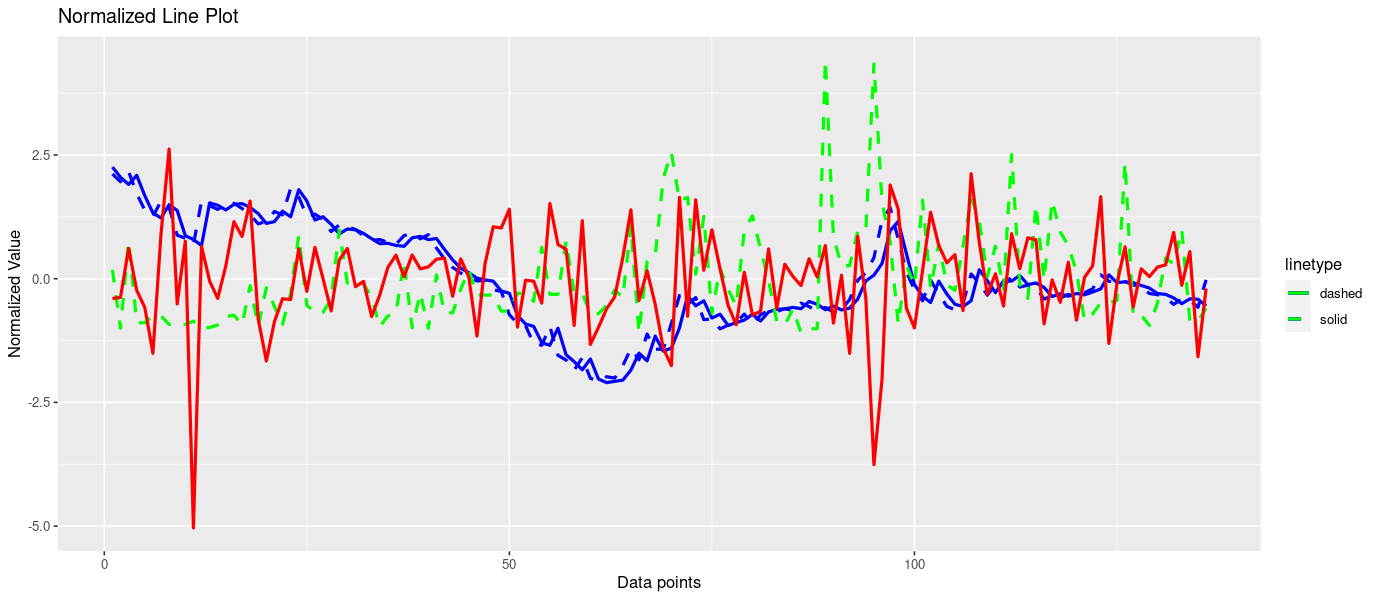
\includegraphics[width=1\linewidth]{MEF_dpdy_MAI_cr.png}
    \caption{Shiny app variable selection outcome, case 1.- \href{https://baumender11.shinyapps.io/Alpha/}{Interactive Shiny App}}
\end{figure}

\noindent In the first case, MEF\_dp and MEF\_dy, MAI\_cr, Quarterly, and 1.1.1985 to 31.12.2018 are selected. Four lines are shown as the outcome. The blue dashed line is from MEF\_dp, the blue solid line is from MEF\_dp + MEF\_dy, and the green dashed line is from MAI\_cr. 

\begin{figure}[H]
    \centering 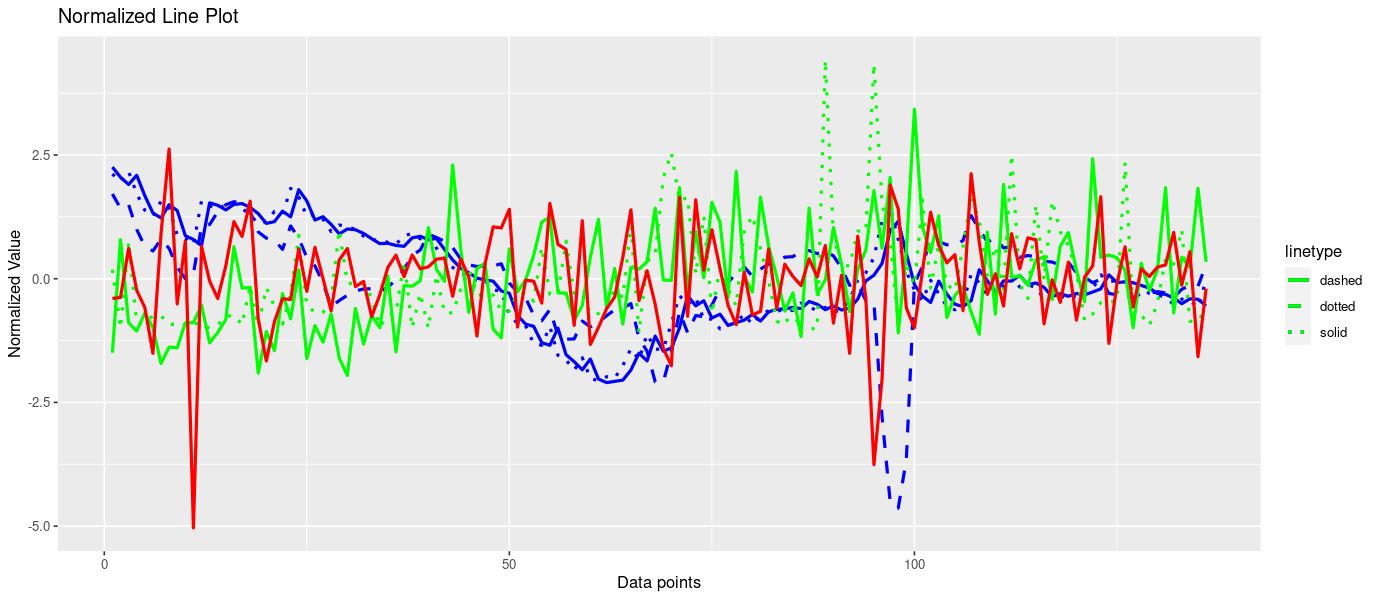
\includegraphics[width=1\linewidth]{MEF_dpdyep_MAI_crgdp.png}
    \caption{Shiny app variable selection outcome, case 2.- \href{https://baumender11.shinyapps.io/Alpha/}{Interactive Shiny App}}
\end{figure}

\noindent In the second case, MEF\_dp, MEF\_dy, and MEF\_ep, MAI\_cr and MAI\_gdp, Quarterly, and 1.1.1985 to 31.12.2018 are selected. Six lines are shown as the outcome. The blue dotted line is from MEF\_dp, the blue solid line is from MEF\_dp + MEF\_dy, the blue dashed line is from MEF\_dp + MEF\_dy + MEF\_ep, the green dotted line is from MAI\_cr, and the green dashed line is from MAI\_cr + MAI\_gdp. 

\noindent Comparing the two cases, a conspicuous observation emerges: the inclusion of the ep variable in an MEF model and the incorporation of the "gdp" variable in an MAI model distinctly enhance the model's proficiency in capturing fluctuations. The predictive accuracy of the model in determining directional movements is notably improved.

\noindent The \href{https://baumender11.shinyapps.io/Alpha/}{interactive Shiny app} also helps show the correlation heatmaps of the variables chosen in a certain temporal range.

\begin{figure}[H]
  \centering
  \begin{subfigure}{0.3\linewidth}
    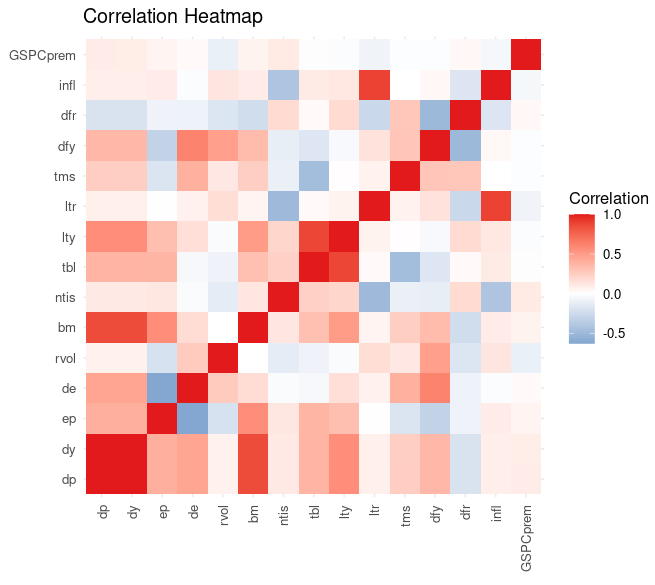
\includegraphics[width=\linewidth]{Cormap_MEF_Daily_85.png}
    \caption{MEF daily.}
  \end{subfigure}
  \hfill
  \begin{subfigure}{0.3\linewidth}
    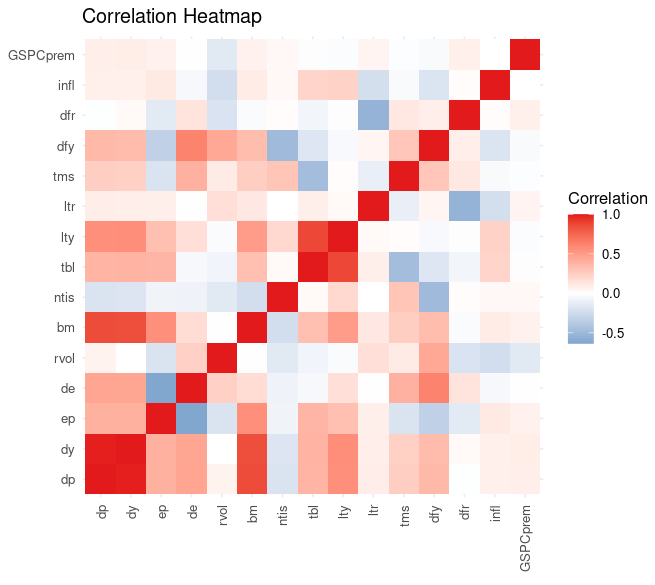
\includegraphics[width=\linewidth]{Cormap_MEF_Monthly_85.png}
    \caption{MEF monthly.}
  \end{subfigure}
  \hfill
  \begin{subfigure}{0.3\linewidth}
    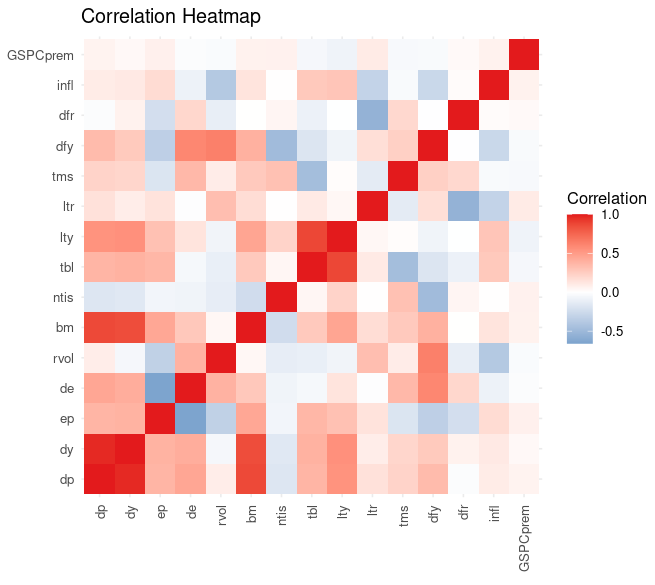
\includegraphics[width=\linewidth]{Cormap_MEF_Quarterly_85.png}
    \caption{MEF quarterly.}
  \end{subfigure}
  \caption{Correlation heatmaps, MEF variables, 1985-2018}
  \label{fig:cormap1}
\end{figure}

\begin{figure}[H]
  \centering
  \begin{subfigure}{0.3\linewidth}
    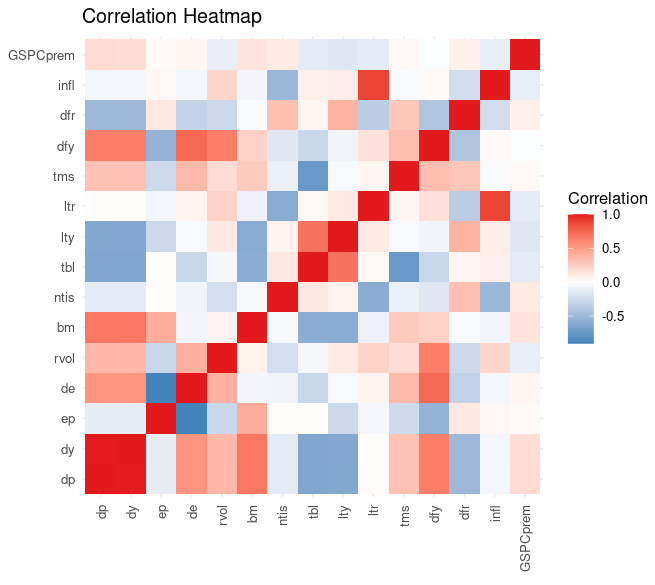
\includegraphics[width=\linewidth]{Cormap_MEF_Daily_00.png}
    \caption{MEF daily.}
  \end{subfigure}
  \hfill
  \begin{subfigure}{0.3\linewidth}
    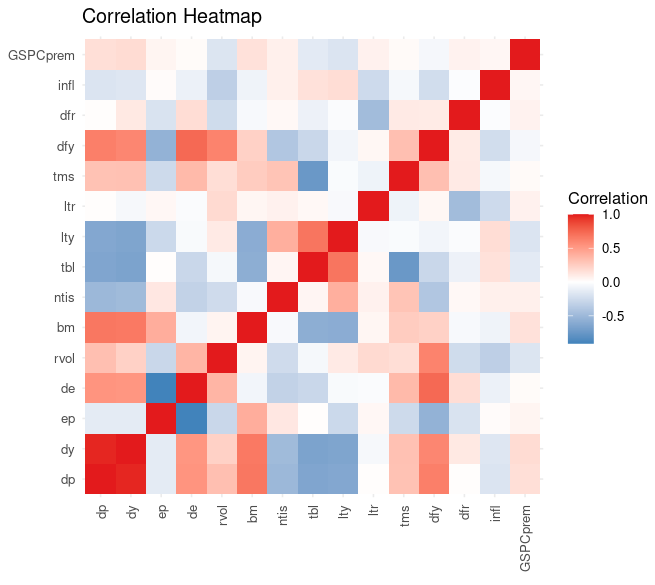
\includegraphics[width=\linewidth]{Cormap_MEF_Monthly_00.png}
    \caption{MEF monthly.}
  \end{subfigure}
  \hfill
  \begin{subfigure}{0.3\linewidth}
    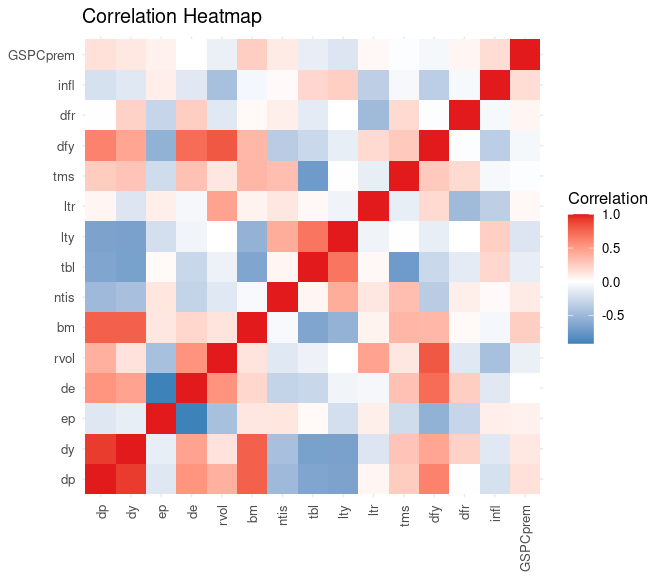
\includegraphics[width=\linewidth]{Cormap_MEF_Quarterly_00.png}
    \caption{MEF quarterly.}
  \end{subfigure}
  \caption{Correlation heatmaps, MEF variables, 2000-2018}
  \label{fig:cormap2}
\end{figure}

\noindent Examining the heatmaps spanning the periods 1985-2018 (Figure \ref{fig:cormap1}) and 2000-2018 (FIgure \ref{fig:cormap2}) reveals a discernible shift in the relevance among certain variables, transitioning from positive (indicated by red hues) to negative (indicated by blue hues). Nevertheless, when scrutinizing distinct frequencies within the identical temporal span, namely daily, monthly, and quarterly data, negligible disparities are evident in the correlation patterns of the variables.

\newpage

\section{Discussion}

\subsection{Practical Implications}

This investigation not only demonstrates the heightened predictive efficacy of neural network models in contrast to linear models but also indicates that utilizing either MEF data or MAI data as input yields comparable impacts on prediction quality, which is different from the conclusions in previous works.

\subsection{Limitations}

While the mean root mean square error (RMSE) of neural network models appears superior to that of linear models, a noteworthy observation is the substantial variability in the RMSE values. For instance, in the case of the neural network model applied to the MAI monthly data, the standard deviation is notably high at 6.056 within the 10 train-test splits, as evident in the accompanying figure.
\begin{figure}[H]
    \centering 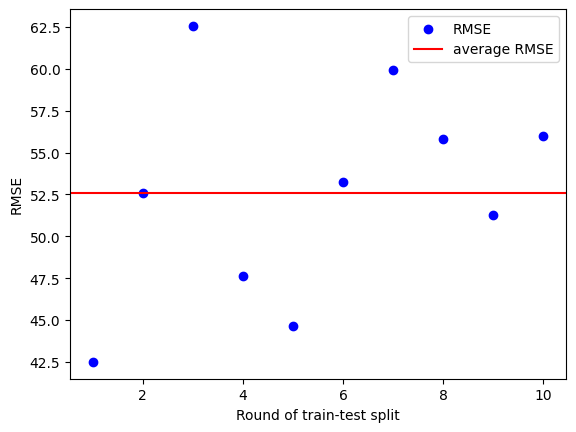
\includegraphics[width=0.7\linewidth]{RMSE of each round of train-test split.PNG}
    \caption{RMSE of each round of train-test split, NN on MAI monthly}
\end{figure}
\noindent The model's performance exhibits a notable dependence on the characteristics of the input data. Despite the random partitioning of ten sets of training and test data within the same dataset, significant variations persist. This variance implies an irregular distribution of the data itself, making the identification of causal relationship patterns challenging. It can be inferred that certain equity risk premia exhibit a more pronounced correlation with the input indices than others.

\subsection{Future Research Directions}

On one hand, there exists ample room for improvement in the model structure. Drawing insights from prior research, it is evident that variables such as equity risk premia often manifest time series correlation characteristics. Our models, which rely solely on macroeconomic features as input, are deemed overly simplistic for robust equity risk premia forecasts. Consequently, the suggestion arises that the initiation of a more formidable modeling approach, beginning with neural network models, would be prudent, with macroeconomic features serving as valuable contributors to the predictive framework.

On the other hand, it is equally valuable to explore scenarios wherein MAI and MEF exhibit noteworthy distinctions in capturing the influence of macroeconomic factors on equity risk premia. This exploration can provide deeper insights into the nuanced dynamics between different macroeconomic indicators and their impact on stock market outcomes.

\newpage

\section{Conclusion}

\subsection{Summary of Findings}

The findings underscore the considerable superiority of neural network models over their linear regression counterparts across diverse datasets. While linear models offer valuable insights into the impact of individual factors on equity risk premia through coefficient examination and significance testing, the predictive strength of neural networks positions them as more robust tools for real-world applications.

Based on previous research, this study has eight models trained—comprising a linear regression model and a neural network model trained on three distinct datasets—to forecast equity risk premia. The performance metrics of these forecasts are presented in a lucid manner.

This study not only emphasizes the heightened predictive efficacy of neural network models but also reveals that the utilization of either MEF data or MAI data as input yields comparable impacts on prediction quality. This stands in contrast to conclusions drawn in prior works, suggesting nuanced considerations in feature selection for equity risk premia forecasts.

\subsection{Limitations and Caveats}

Despite the overall superiority of neural network models, an important consideration is the observed variability in RMSE values. The model's performance exhibits dependence on input data characteristics, indicating an irregular data distribution and the challenge of identifying causal relationship patterns.

\subsection{Recommendations for Future Research}

Further exploration is warranted in enhancing the model structure, acknowledging insights from previous research indicating time series correlation characteristics in equity risk premia. A recommendation is made to explore more sophisticated modeling approaches, commencing with neural network models and incorporating macroeconomic features as valuable contributors to the predictive framework.

Additionally, investigating scenarios where MAI and MEF exhibit distinctions in capturing the influence of macroeconomic factors on equity risk premia presents an avenue for future research. 

\newpage

\section{References}

\patchcmd{\thebibliography}{\section*{\refname}}{}{}{}

\begin{thebibliography}{9}
\bibitem{Fama1988}
\href{https://www.sciencedirect.com/science/article/pii/0304405X88900207}{Fama and French (1988). \emph{Dividend Yields and Expected Stock Returns}.}

\bibitem{Goyal2003}
\href{https://www.jstor.org/stable/4133989}{Goyal and Welch (2003). \emph{Predicting the Equity Premium with Dividend Ratios}.}

\bibitem{Lo2021}
\href{https://www.tandfonline.com/doi/full/10.1080/14697688.2023.2203844}{Lo and Singh (2003). \emph{Deep-learning models for forecasting financial risk premia and their interpretations}.}

\bibitem{Gu2019}
\href{https://dachxiu.chicagobooth.edu/download/ML.pdf}{Gu, Kelly, and Xiu (2019). \emph{Empirical Asset Pricing via Machine Learning}.}

\bibitem{Andrei2012}
\href{https://www.epfl.ch/labs/cfi/wp-content/uploads/2018/08/WP757_A2.pdf}{Andrei and Hasler (2012). \emph{Investors’ Attention and Stock Market Volatility}.}

\bibitem{Nikkinen}
\href{https://www.sciencedirect.com/science/article/pii/S104402830600024X}{Nikkinen, Omran, Sahlström, and Äijö (2006). \emph{Global stock market reactions to scheduled U.S. macroeconomic news announcements}.}

\bibitem{Ma2022}
\href{https://doi.org/10.1016/j.intfin.2022.101603}{Ma, Lu, Liu, and Huang (2022). \emph{Macroeconomic attention and stock market return predictability}.}

\end{thebibliography}

\newpage

\section{Appendices}
% Additional information or supplementary material.

\end{document}
